\clearpage
\section{Fagligt vidensgrundlag}

Vidensgrundlaget for udarbejdelsen af denne rapport gennemgås i dette afsnit, med redegørelse for relevante begreber, teori samt det faglige vidensgrundlag. Dette afsnit tager udgangspunkt i det tilsvarende afsnit fra inceptionsdokumentet med tilføjelser samt udbedringer. 
Gruppens viden og færdigheder omkring udviklingen af software programmet, samt metode og planlægning, bygger på det lærte indhold fra de øvrige fag på 2. semester. 

\subsection{Kravudvikling}

Når kravene til et system skal findes vil man som regel følge et workflow, der sikrer at kravene bliver så præcise, komplette og konsistente som muligt. 
\begin{itemize}
    \item Præcise krav, da tvetydige krav kan fortolkes på forskellige måder. 
    \item Komplette krav, så de indeholder beskrivelser af alle aspekter. 
    \item Konsistente krav der er konsekvente. Kravene må altså ikke modsige hinanden eller være i konflikt med hinanden.
\end{itemize}
Kravene til et softwaresystem er derfor vigtige at have styr på, da de fastsætter hvad systemet skal gøre, og definerer begrænsninger for dets udvikling og drift. 


For at få et optimalt workflow til at få skabt nogle gode krav, har vi i gruppen kigget på at lave en brugsmønstermodel, også kaldet use-case. 
Det indebærer, at vi først har fundet de aktører, der forbindes med systemet. For at identificere en aktør kan man spørge: "Hvem eller hvad bruger systemet?" "Til hvad?" og "Hvorfor?". Man kan kigge på hvilken rolle de spiller i interaktionen med systemet. Man kan også spørge, hvilke andre systemer bruger eller bidrager med til systemet. Når man er afklaret med hvilke aktører der er, skriver man dem op i listeformat, hvor man inkluderer aktørernes navne, deres mål (hvad og hvorfor) og deres bidrag.

Næste punkt i en brugsmønster-model er at finde og identificere brugmønstre.
Når man identificerer brugsmønstre vil man gå ud fra listen over aktører, og stille sig selv en række spørgsmål. Hvilke mål har en aktør? Det er skrevet ned i listen, og man kan derfor lave et brugsmønster til hvert mål aktøren har. Hvilke funktioner vil en specifik aktør have af systemet? Til det kan man lave et brugsmønster til en funktion, der giver målbare resultater til aktøren. Gemmer systemet information, som den henter frem? I så fald, for hvilken aktør gør den det? Dette er også værd at overveje, når vi skal lave brugsmønstrene. Ligeledes som med aktørerne, laver vi en liste over brugsmønstre, der indeholder deres navne og deres formål.
Til slut skal der identificeres systemgrænser. Til det skal der først tegnes et brugsmønster diagram med aktører, de fundne brugmønstre, og linjer herimellem, der forbinder aktøren med de relevante brugsmønstre. Nu er det vigtigt, at man evaluerer, sine brugsmønstre, aktører og emnet. Ud fra sine evalueringer kan man nu danne sig et billede af, hvilke krav, der stilles til systemet, og man ender derfor med en skitsering af en kravspecifikation til systemet.


\subsection{Analyse af brugsmønstre}
Brugsmønstrene kan vi derefter analysere og udarbejde sekvensdiagrammer og operationskontrakter, som vi kan overføre til et klassediagram og derved opbygge et overblik over systemet. 

Dette foregår ved at der bliver udvalgt en række brugsmønstre til analysen. Til hvert af disse udformes et sekvens diagram, som viser det specifikke hændelsesforløb indefor et brugsmønster og de objekter og den adfærd der er beskrevet i brugsmønsteret. 

Ud fra skevens diagrammet laves en operationskontrakt, som beskriver de forpligtigelser operationen har, samt hvilke ændringer der forekommer i systemet efter operationen er kaldt. 

Dernæst kan et systemsekvens diagram udarbejdes. Et systemsekvens diagram er et udvidet sekvensdiagram, som viser den komplette række af begivenheder der udføres når operationen udføres. Til sidst kan det udvidet sekvens diagram overføres til et klassediagram. 


\subsection{Arkitektonisk design}
Arkitekturen for systemet fastlægges tidligt i elaborationsfasen, når det er Unified Process der bliver benyttet. Det er vigtigt for ethvert software projekt at systemets arkitektur er velovervejet og godt udarbejdet, da det vil få stor betydning for det endelige produkt kvalitet. Designet fastlægges hovedsaligt ud fra de ikke-funktionelle krav, som f.eks. at vi i dette projekt har et krav om en tre-lags arkitektur, der allerede har sat bestemte rammer for det arkitektoniske design. 


\subsection{Brug af SCRUM i projektet}
SCRUM er et agilt projektudviklings værktøj der primært er udviklet til udviklingen af software. SCRUM bygger overordnet på 3 artefakter. Product backlog, sprint og inkrementer. 

\paragraph{Product backlog}
Product backlog er en liste af opgaver/krav der skal implementeres på et produkt for at nå et fælles produktmål. Emnerne i product backlog er prioriteret således at det mest nødvendige implementeres først. Disse emner er hvad der indgår i det næste SCRUM artefakt, sprintet.

\paragraph{Sprint}
Et sprint er en plan for at implementere en mængde af krav, for at opnå et mål. Man deler sprintplanlægningen op ved at besvare følgende spørgsmål om det. hvorfor, hvad og hvordan. Ved at finde ud af hvad målet for sprintet er, har man hvorfor sprintet er vigtigt. Derefter vælges de emner i product backlog, der, når implementeret, opnår dette mål. Disse emner sættes ind i et såkaldt sprint backlog der fungerer på samme måde som product backlog, blot kun for et sprint. Dette sprint backlog er også prioritet er derved har man en plan for sprintet, og derved besvaret hvordan.

\paragraph{Inkrement}
Et inkrement er et betydeligt skridt på vej hen mod det endelige produkt. Et inkrement skal præsentere en virkende del af programmet. Det vil sige der hele vejen igennem er et kørende program, der udbygges med features inkrement efter inkrement. 

SCRUM benytter sig også af nogle roller, der er essentielle for succesfuld brug af værktøjet. 

\paragraph{SCRUM master}
En SCRUM master står får at få etableret SCRUM-flowet. Dette gøres ved at de skaber en fælles forståelse for hvordan arbejdsprocessen ser ud, og hvilket værktøjer der anvendes og hvordan. Det er SCRUM masterens opgave at sørge for hele processen bliver overhold, for hvis ikke dette formås, forsvinder alle fordelene ved SCRUM. 
I Gruppen har Hans Pedersen ageret som SCRUM master

\paragraph{Product owner}
En product owner er ansvarlig for product backlog. Det er vigtigt at de emner der skal op på product backlog, går gennem product owner, så de har det fulde overblik over hvad produktet indeholder. Derfor er der også kun én product owner, så man sikrer sig at der altid er en der har 100\% styr på hvordan produktet ser ud, og hvordan det skal se ud. Idet gruppen er lille nok til kun at indeholde et SCRUM team, har gruppen udnævnt at product master er hovedansvarlig for produktet. 
I gruppen har Jonas Beltoft ageret som product owner, da han er iderig, og har gode evner indenfor programmering, og visualisere sig programmer.

\paragraph{Developers}
Developers, eller udviklere, er dem der sørger for at et sprint rent faktisk også arbejder fremad mod et inkrement. De står for at implementere de emner der er tilføjet til sprint backlog
I gruppen er alle medlemmer indgået som udviklere.

\subsection{Objekt-orienteret programmering}
\paragraph{Hvad er OOP?}
Objekt-orienteret programmering (eller OOP), er et programmeringsparadigme baseret på et koncept af "objekter". Disse objekter kan indeholde en række data, generelt kaldet attributter. Kode kan være skrevet i form af en procedure, der skal lave noget bestemt, dette bliver kaldt en metode. Et eksempel kunne være at kode en person, denne person ville være et objekt. Personen har flere forskellige metoder til at kunne tale, bevæge sig, trække vejret OSV. Person objektet skal også have nogle attributter så som en højde, deres køn, deres alder osv. 

Ved brug af Java-kodesprog i dette projekt kommer vi til at gøre stor brug af klasser. Når man definerer en klasse, opretter man egentlig et blueprint til et objekt. Heri defineres ikke direkte data, men der defineres hvad der skal gøres med noget data der er givet til objektet.

\subsubsection{OOP's fire basale koncepter }

    \paragraph{Indkapsling}
    Når man snakker om indkapsling inden for OOP, så betyder det at nogle data eller noget funktionalitet bliver indkapslet. Dette gøres ved hjælp af Access modifiers. Access modifiers hjælper til at bestemme, hvem der har adgang til data og funktioner, og hvor meget der er adgang til. Der findes en række forskellige access modifiers som kan ses på tabellen \ref{tab:Access modifier} på side \pageref{tab:Access modifier}. Indkapsling er en god måde at lave dataskjulning for andre klasser. Indkapsling gør det også nemmere at teste produktets sikkerhed. 
        
        \begin{table}[H]
        \centering
            \begin{tabular}{p{2cm}|p{2cm}|p{2cm}|p{3cm}|p{2cm}}
                \textbf{Access Modifier} & \textbf{Inden for klassen} &
                \textbf{Inden for pakken} & \textbf{Uden for pakken kun af
                subklasser} & \textbf{  Uden for pakken} \\
                \hline
                Private   & X &   &   &   \\
                \hline
                Default   & X & X &   &   \\
                \hline
                Protected & X & X & X &   \\
                \hline
                Public    & X & X & X & X \\
            \end{tabular}%
            \caption{Liste over tilgange ved de forskellige access modifiers}
            \label{tab:Access modifier}
        \end{table}

    \paragraph{Abstraktion}
    Abstraktion er en måde på at gemme specifikke værdier og metoder. Abstraktion kan ses som en udvidelse på indkapsling, siden det kan gemme information eller metoder for ekstern kode. Dette gør interfacet af objekter meget simpelt. F.eks. kan abstraktion forstås ved at kigge på kroppen, vores skind fungere som an abstraktion til at gemme hvad der foregår inde i kroppen.

    \paragraph{Nedarvning}
    Nedarvning kommer fra at være en subklasse. Her nedarver subklassen attributter og metoder fra dens superklasse. Dette gøre det muligt at nemmere kunne genbruge kodestykker. Derudover bruges det også til metodeoverskrivning så man kan opnå runtime polymorfi. 
    Imodsætning til nedarvning, hvilket er it såkaldt "IS-A" forhold, findes der også et "HAS-A" forhold, et aggregat.
    Et HAS-A forhold beskriver de gange hvor et objekt gøre brug af et andet objekt til at gemme data. F.eks. hvis man har en kunde med nogle informationer inde i et objekt, så kan der herunder oprettes et adresse objekt hvilket indeholder information som by, kommune, post nummer osv. 
    Et aggregat kan være god at bruge i situationer hvor en stor klasses information kan deles ud i mindre bidder.  Det hjælper også meget på kode genanvendelse.
    I den virkelige verden kan vi forestille os nedarvning ved at kigge på insekter. Alle insekter har lignende egenskaber så som at have seks ben eller et exoskelet. Altså ville en grasshoppe eller myre have nedarvet disse egenskaber fra superklassen af insekter.
    \paragraph{Polymorfi}
    Polymorfi er muligheden for at et objekt kan tage flere former. Dette gør at vi kan implementere en metode fra en superklasse i en subklasse på forskellige måder. 
    Det ville altså sige at hvilket som helst subklasse objekt i Java kan hvilken som helst form som er i superklassens hierarki, inkluderende sig selv.
    Generelt er der to typer af polymorfi:
    \begin{itemize}
        \item Dynamisk polymorfi 
        \subitem 
        Dynamisk polymorfi er også kendt som run-time polymorfi. Dette kan beskrives ved at tænke på superklasse-subklasse forhold. De begge har den samme metode, og subklassen har overskrevet superklassens metode (metode overskrivelse).
        Når et objekt bliver tildelt en klasse reference, og en metode fra objektet bliver kaldt, så er det metoden indeni objektets klasse, der bliver udført. Der bliver altså ikke kaldt metoden fra reference klassen, hvis altså referencen er en superklasse. %skal lige læses igennem, der er nogle lange sætninger
        \item Statisk polymorfi 
        \subitem Statisk polymorfi er  også kendt som compile-time polymorfi eller metode overbelastning. Dette betyder, at man har angivet flere af de samme metodenavne, men med forskellige argumenter. Det betyder altså, når man kalder sådan en metode, så ville kompilatoren beslutte hvilken metode, der bliver kørt i forhold til hvilke parametre, der er angivet.
    \end{itemize}
    
\subsection{Trelagsarkitektur}
Trelagsarkitekturen er en softwarearkitektur, der deler programmet op i tre lag. Et præsentationslag, et logiklag og et datalag: 
\begin{itemize}
    \item Et præsentationslag som udelukkende står for at forsyne brugeren med en brugerflade og hente information fra brugeren og med den information kommunikere med det næste lag, logiklaget.
    \item Logiklaget (også kaldet domænelaget) står for alle de logiske operationer som er associeret med de gældende elementer i præsentationslaget på baggrund af den information, som brugeren har indtastet. Logiklaget kommunikerer også med datalaget, og kan her sammenholde information fra brugeren med det i databasen for at tage en beslutning om, hvad programmet skal gøre.
    \item Datalaget står for at lagre systemets data som logiklaget kan anvende.
\end{itemize}

Figur \ref{fig:trelagsarkitekur} beskriver denne lagdeling. 

\begin{figure}[H]
    \centering
    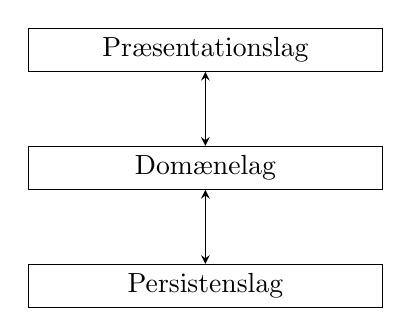
\begin{tikzpicture}
        \node[rectangle, draw, minimum width=4.5cm] (presentation) at (0,0) {Præsentationslag};
        \node[rectangle, draw, minimum width=4.5cm] (domain) at (0,-1.5) {Domænelag};
        \node[rectangle, draw, minimum width=4.5cm] (persistenslag) at (0,-3)
            {Persistenslag};
        \draw[stealth-stealth] (presentation) -- (domain);
        \draw[stealth-stealth] (persistenslag) -- (domain);
    \end{tikzpicture}
    \caption{Beskrivelse af en trelagsarkitektur}
    \label{fig:trelagsarkitekur}
\end{figure}

For en succesfuld anvendelse af trelags arkitekturen vil brugeren udelukkende
blive præsenteret for præsentationslaget og behøver ingen viden om de
underliggende lag, da al kommunikation mellem bruger og program sker i dette
lag. Brugen af trelags arkitekturen giver nogle fordele. 
\begin{itemize}
    \item Først og fremmest kan udarbejdelsen af de forskellige lag uddelegeres
        således at de udvikles samtidig. Dette gør udviklingen af programmet
        hurtigere 
    \item Da al logikken sker et sted, bliver programmet mere
        skalérbart idet at koden/programmet ikke er kludret sammen og har for
        mange indgangspunkter.  
    \item Hvis et lag bryder sammen eller ikke
        virker, påvirkes de andre ikke, da de er opdelt.
    \item Grundet at trelags arkitekturen opdeler præsentationslaget og
        datalaget med et logiklag, vil man med korrekt implementering kunne
        sikre, at en bruger ikke får tilladelse til at tilgå data, som ikke er
        tiltænkt dem. 
    \item Lagdelingen bevirker at man kan ændre på implementeringen af et givent
        lag uden at de andre bemærker det.
\end{itemize}

\subsection{Unified Process} \label{section: Unified Process}
Unified Process (UP) er en iterativ og trinvis udviklingsproces. UP er delt op i 4 trin, eller faser, disse og deres definitioner er:
\begin{itemize}
    \item Inceptionsfasen
        \subitem I inceptionsfasen skal man finde ud af projektets gennemførlighed, finde frem til vigtige krav og identificere potentielle risici.
    \item Elaborationsfasen
        \subitem I elaborationsfasen skal der laves en arkitekturprototype, oveni at risikovurderingen forbedres. Hertil skal hovedparten af brugsmønstrene findes, samt at der skal lægges en plan for konstruktionsfasens forløb.
    \item Konstruktionsfasen
        \subitem I konstruktionsfasen færdiggøres den endelige identifikation af brugsmønstre, samt disses beskrivelse og realisering. Analyse, design, implementation og test færdiggøres også i denne fase. Undervejs redigeres projektets risikovurdering.
    \item Transitionsfasen
        \subitem I denne fase rettes fejl, og brugerne forberedes på at anvende softwaren. Her laves også manualerne og anden dokumentation, til sidst gennemføres et review af projektet. 
\end{itemize}
 
En vigtig pointe omkring UP er at det er en proces drevet af brugsmønstre (use cases), samt at der fokuseres på risikostyring og arkitektur. Og som tidligere nævnt er der fokus på iterationer og en trinvis udviklingsprocess. Dette betyder at systemet udvikler sig trinvist for hver iteration.


\subsection{UML}

UML eller Unified Modeling Language, tilbyder en måde at visualisere et systems arkitekturelle blueprints i et diagram. 

\subsubsection{Klassediagrammer}

Det er bl.a. brugt til at lave Class Diagrams, da det giver en oversigt over hvilke klasser der er i et program, hvilke attributter og metoder de har, samt disses synlighed (Access Modifiers). UML anfører også sammenhængen mellem klasserne, om de fx nedarver fra klassen eller andet, hvilket er en stor del af grunden til at man bruger UML.  Ud fra det kan man aflæse hvordan forskellige klasser bliver brugt andre steder i programmet, og derved få en bedre forståelse for hvordan programmet virker, uden at man har set programmet køre. Der er særlig notation til at fremhæve alle OOP's fire basale koncepter, 

\begin{wrapfigure}{r}{0.26\textwidth}
    \vspace{0cm}
    \begin{tikzpicture}
        \umlclass{Kunde}{
        \small - navn: String\\
        \small - email: String\\
        \small- saldo: long\\
        \small- kurv: Vare[]\\
        }
        {
        \footnotesize+ Kunde()\\
        \footnotesize+ tilføjTilKurv(Vare) : void\\
        \footnotesize+ købVarerIKurv() : Vare[]\\
        }
        \umlclass[y=-5.5]{Vare}{
        - navn: String\\
        - pris: Double\\
        - udløbsdata: Date\\
        }{
        + Vare()\\
        }
        \umlcompo{Kunde}{Vare}
    \end{tikzpicture}
   % \centering
    %\includegraphics[width = 0.25\textwidth]{Images/UML eksempel.png}
  \caption{UML klassediagram for sammenhængen mellem en Kunde og en Vare}
  \label{fig:UML eksempel}
\end{wrapfigure}  

hvilket gør det muligt at udarbejde og/eller visualisere præcist det program, der er ønsket. Øverst ses navnet på den klasse, der beskrives. I sektionen under, er alle klassens attributter, og under dem er klassens metoder. Hvis klassen har en eller flere constructors, kan disse også ses, da de har det samme navn som klassen. På grund af alt dette, kan UML være et meget kraftfuldt værktøj under udviklingen af et objektorienteret program, da man kan visualisere alle de objekter og klasser, der bliver lavet og instantieret. Samt sammenhængen mellem disse objekter og klasser. UML bruges også til andre ting, såsom brugsmønster-diagrammer, som giver et overblik over aktører og de brugsmønstrer de interagerer med. Dette er en anderledes måde at modellere på, men det er alt sammen under UML, da det er en universel måde at forbinde elementer på, i en visuel kontekst.


\subsubsection{Beskrivelse af database med UML}
UML kan også bruges til at vise en database. Det ses nemt hvilken udgave, der er brugt, da man her vil se notationer så som \{PK\} som beskriver at denne attribut er en primær nøgle i denne tabel. Hver kasse er her ikke en klasse, men en tabel. Den har kun attributter, da en tabel ikke har funktioner. Et UML diagram over en database vil også have forskellige måder at visualisere sammenhæng mellem tabellerne.
Klassediagrammet som beskrevet har kun én standardiseret måde at forbinde klasserne på, hvilket gør det nemmere at lære og hurtigere at finde ud af, hvad der menes med de forskellige symboler man støder på, hvorimod et UML diagram over en database har flere forskellige måder at vise sammenhæng på, selvom de viser det samme. I klassediagrammet vil man se symboler som f.eks. betyder at denne klasse nedarver fra en anden klasse, eller bl.a. viser at den ene klasse "bruger" eller "afhænger" af en anden klasse. Dette finder man ikke i et database UML diagram. Her viser forbindelserne, hvor mange elementer, der kan være, f.eks. kan en kunde købe mange varer, men en type vare kan købes af mange forskellige kunder, så det vil kaldes en mange til mange forbindelse. Dette kan noteres på forskellige måder, f.eks. med crows foot, Chen eller andre. Vi som gruppe vil bruge Chen, som er en meget simpel måde at vise, om det er 0, 1 eller flere. Disse notationsformer er også brugt i ER og EER modeller, men det betyder ikke at et UML diagram er det samme som et ER eller EER diagram, da de ikke går direkte ned i databasen, men er mere en overordnet beskrivelse og kan vise andre ting end UML kan.

\subsection{MoSCoW}
MoSCoW er en model der bruges når en liste af krav skal prioriteres. Kravene indeles i 4 grupper, efter hvor vigtige de er for projektets succes. Her startes der med "Must Have" som er de vigtigste krav og som er nødvendige for at projekt bliver en succes. Dernæst kommer "Should Have" som er krav, der ikke er nødvendige, men det vurderes at de giver en tilstrækkelig værdi til projektet, i forhold til arbejdsindsatsen. "Could Have" er krav som ikke er vigtige for projekts gennemførsel, de kan tages med i tilfælde af overskydende arbejdsressourcer, men der planlægges ikke efter, at de skal medtages. Til sidst findes "Would Have" som er krav, der giver mening for projektet, men er valgt fra i den pågældende udgave af projektet. 

\subsection{FURPS+}

\begin{itemize}
    \setlength\itemsep{0em}
    \item Usability
    \subitem "Usability" handler om de menneskelige interaktioner med programmet. Det gælder om at se på, hvor effektivt programmet er. Er dokumentationen for programmet i orden og uddybende nok, til at forklare hvad programmet står for.
    \item Reliability
    \subitem "Reliability" omhandler det, der vedrører oppetid, præcision i systemets beregninger.
    \item Performance
    \subitem "Performance" drejer sig om, hvordan systemet skal reagere på større mængder af information.
    \item Supportability
    \subitem "Supportability" omhandler krav, som vedrører testbarhed, kompatibilitet, konfigurerbarhed.
    \item Plus
    \subitem "Plus" er den del af FURPS+ der indeholder begrænsninger og specifikke krav for systemet.
    \begin{itemize}
        \item Design constraints
        \subitem Man kigger på designmæssige begrænsninger, der kunne være for projektet. Ændrer I/O enheder eller den valgte DBMS, hvordan softwaren skal bygges?
        \item Implementation requirements
        \subitem Man kigger også på implementationen og dets krav, og beskriver, hvordan programmørene skal forholde sig. Skal de bare forholde sig til standarderne?
        \item Interface requirements
        \subitem Interface krav kigger på om, der er nogle interfaces som programmet skal fungere på eller med.
        \item Hardware requirements
        \subitem Til sidst er der hardware krav, hvor der kigges på, om der er nogle krav til hvilken hardware systemet skal interagere med eller kører på, og om det skaber nogle forudsætninger for produktionen. 
    \end{itemize}
\end{itemize}
